\section{fireMIP}
\pgfdeclareimage[width=1.0\paperwidth]{header-image}{header_images/kata_tjuta}

\begin{frame}[label = kelley2013Datasets]
	\frametitle{ Multi-model scores}
	\framesubtitle{Model scores}
	
	% Smileys
	\foreach \x in {1, 2, 3, 4, 5, 6, 7} {
		\only<\x> {
			\includegraphics[width=10cm]{images/modelScores/pp\x.png}
	}}
	%Fire and veg
\end{frame}

\begin{frame}[label = kelley2013Datasets]
	\frametitle{JULES-INFERNO v obs}
	\framesubtitle{Model scores}
	
	\begin{textblock*}{8cm}(11cm ,1.3cm)
		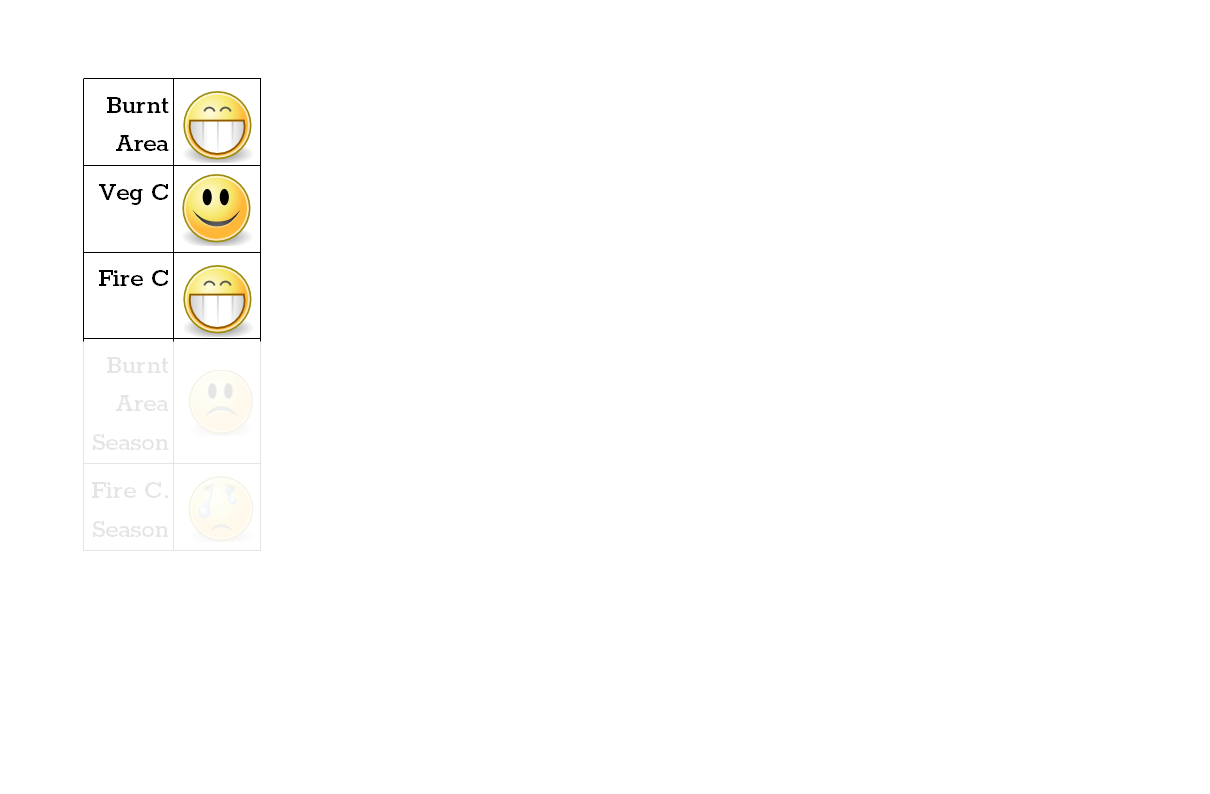
\includegraphics[width=7.5cm]{images/Smileys/BAvegCFireC.png}
	\end{textblock*}
	
	\only<2-> {
		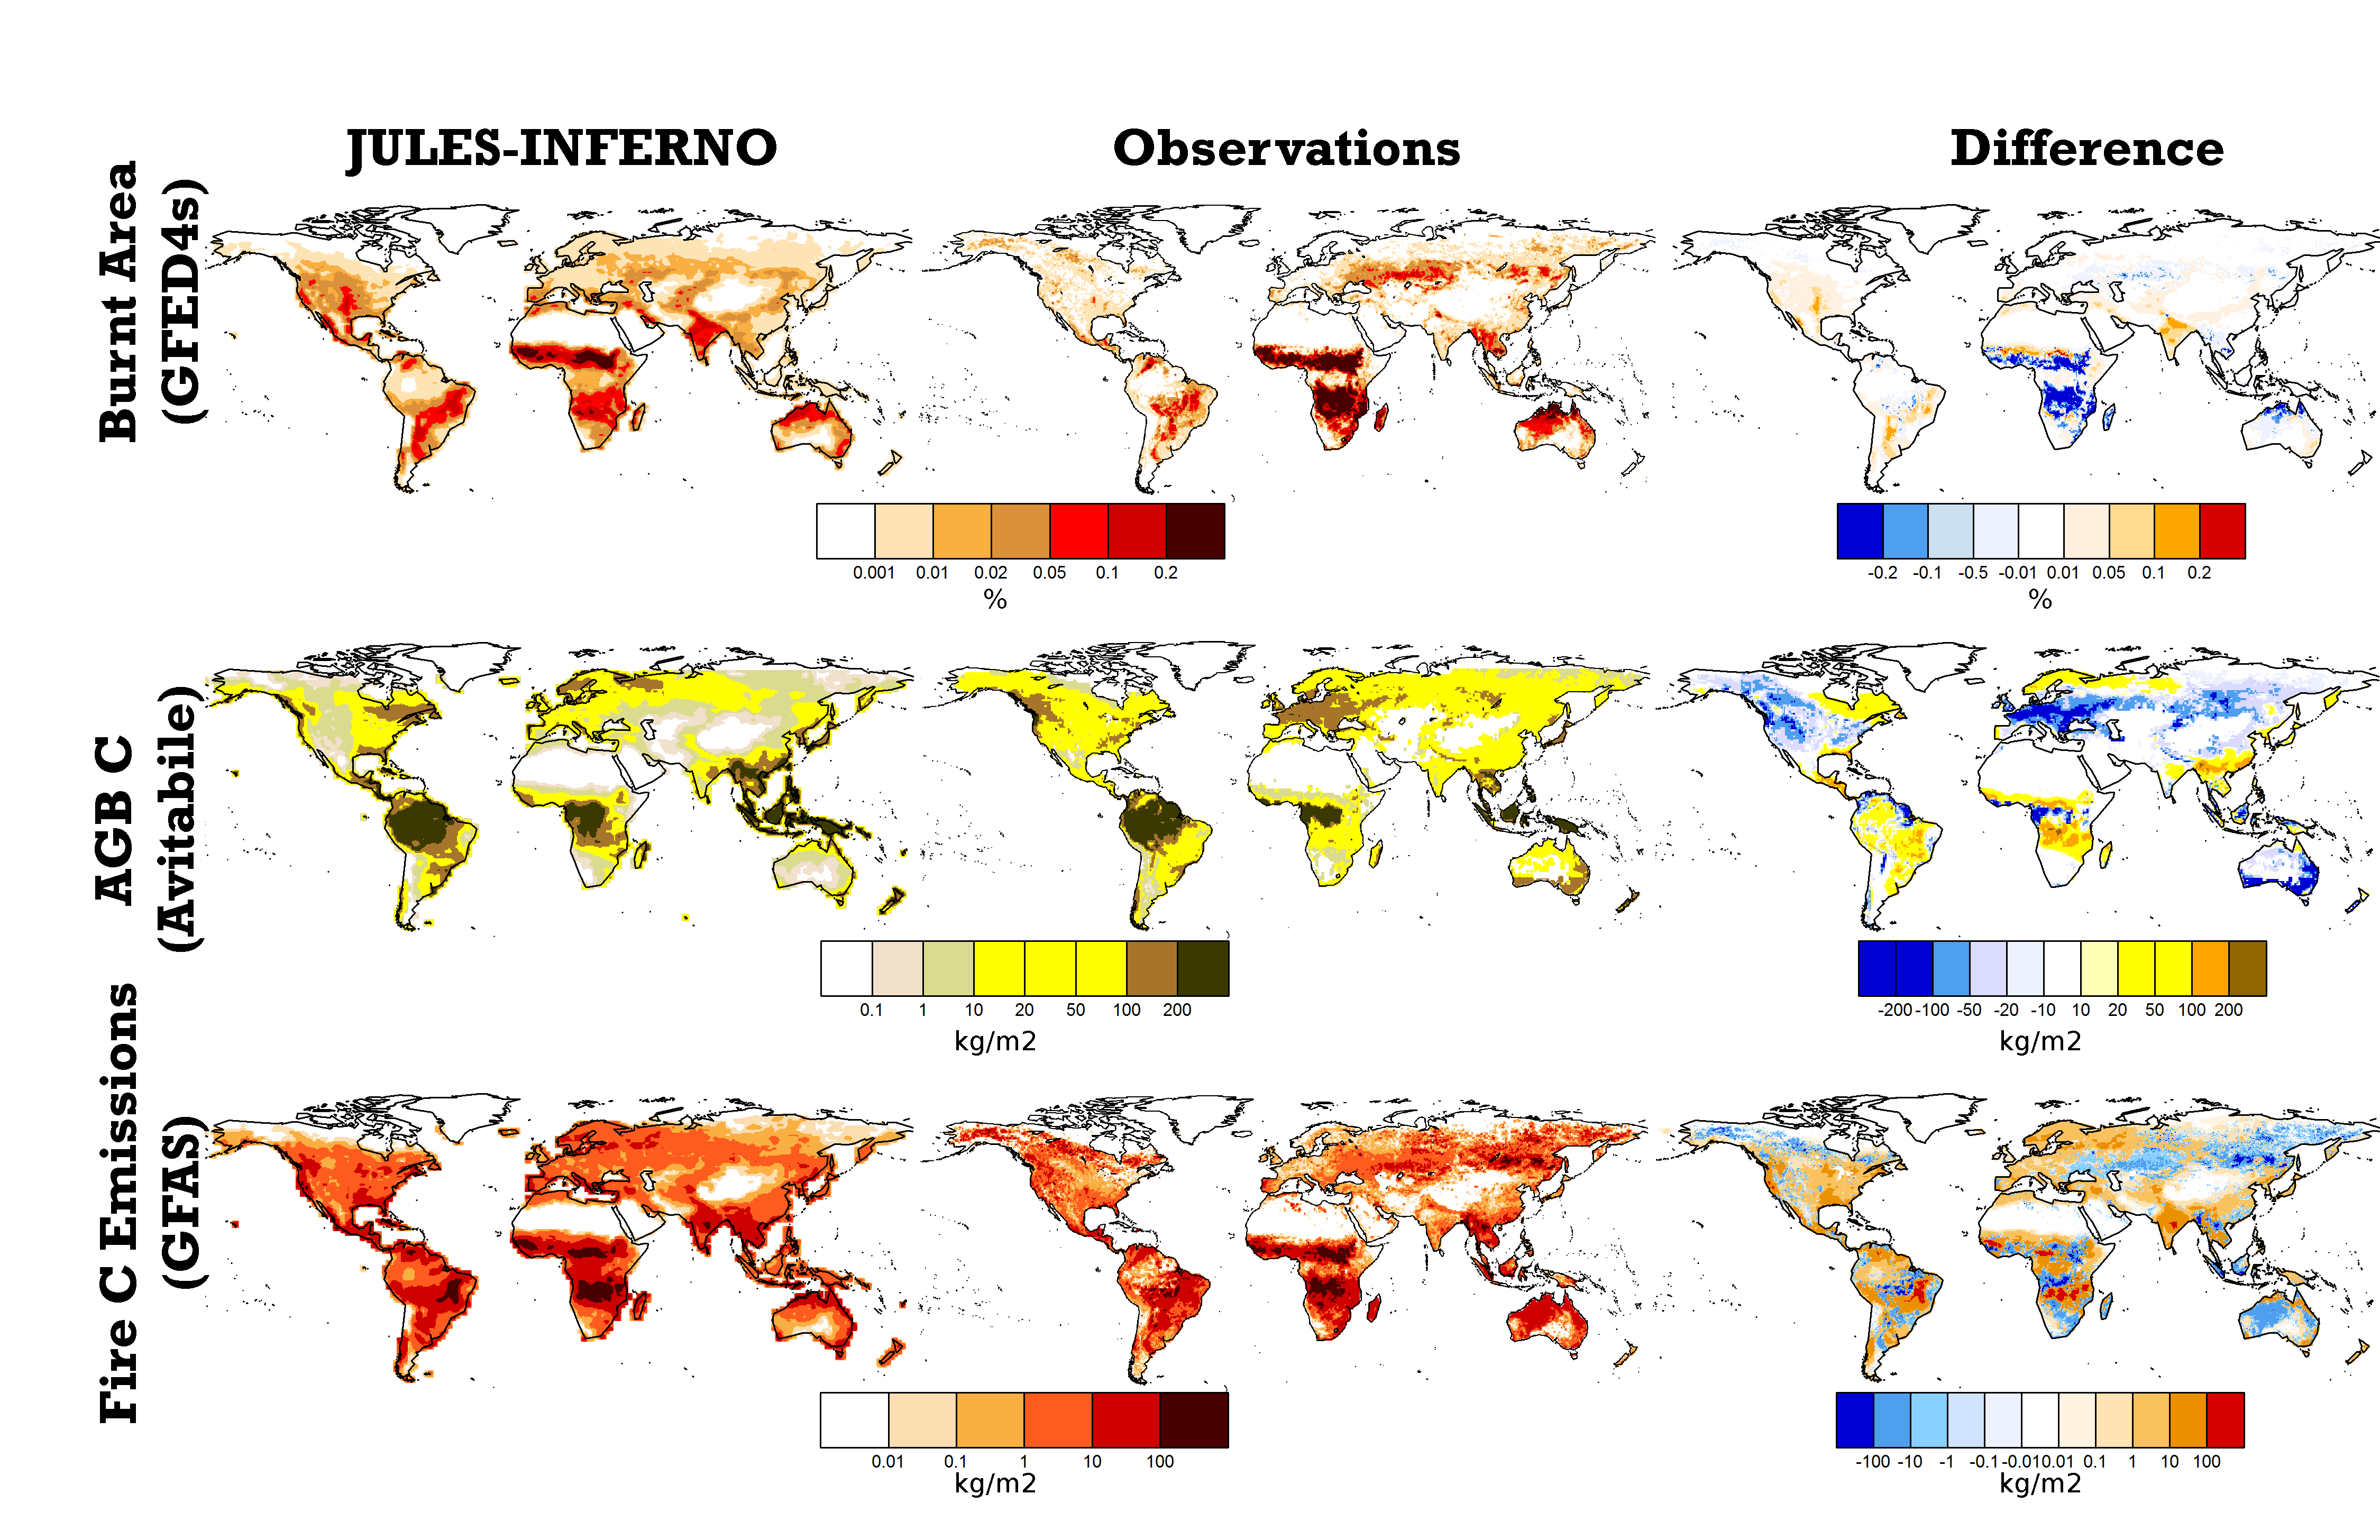
\includegraphics[width=10cm]{images/julesPerformance/FireMapsSpatial.png}
	}
\end{frame}

\begin{frame}[label = kelley2013Datasets]
	\frametitle{Multi-model scores}
	\framesubtitle{Model scores}
	
	\begin{textblock*}{8cm}(11cm ,1.3cm)
		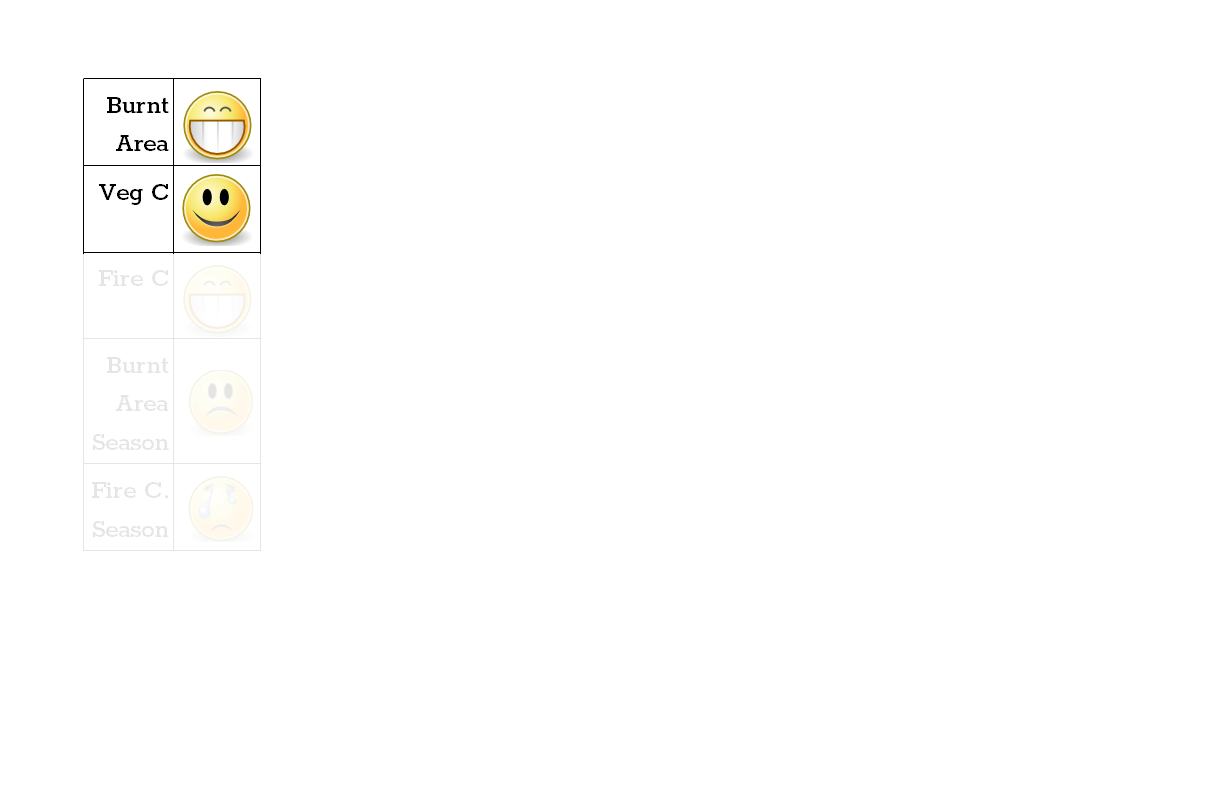
\includegraphics[width=7.5cm]{images/Smileys/BAvegC.png}
	\end{textblock*}
	
	\foreach \x in {1, 2} {
		\only<\x> {
			\includegraphics[width=10cm]{images/fireVsVegScores/pp\x.png}
	}}

\end{frame}

\pgfdeclareimage[width=1.0\paperwidth]{header-image}{header_images/Sierra_Calderona}

\begin{frame}
	\frametitle{It burns where it rains \small{(a bit)}}
	\framesubtitle{Uni-modal relationship with moisture}
	
	
	\begin{textblock*}{14cm}(-0.5cm,1.5cm)
		\begin{tikzpicture}
		
		\foreach \x in {1, 2, 3, 4, 5} {
			\visible<\x-> {
				
				\node[anchor=south west,inner sep=0] (image) at (0,0) {
					\includegraphics[width=13.7cm]{images/unimodal/p\x.png}%images/unimodal/p\x.png}
				};}}
		
		\end{tikzpicture}
	\end{textblock*}
	
	%Make clear we are talking about burnt area
\end{frame}

\begin{frame}
	\frametitle{INFERNO Fire Controls}
	%\framesubtitle{Geographic controls}
	\only<1->{
		\begin{textblock*}{14cm}(0.3cm,1.2cm)
			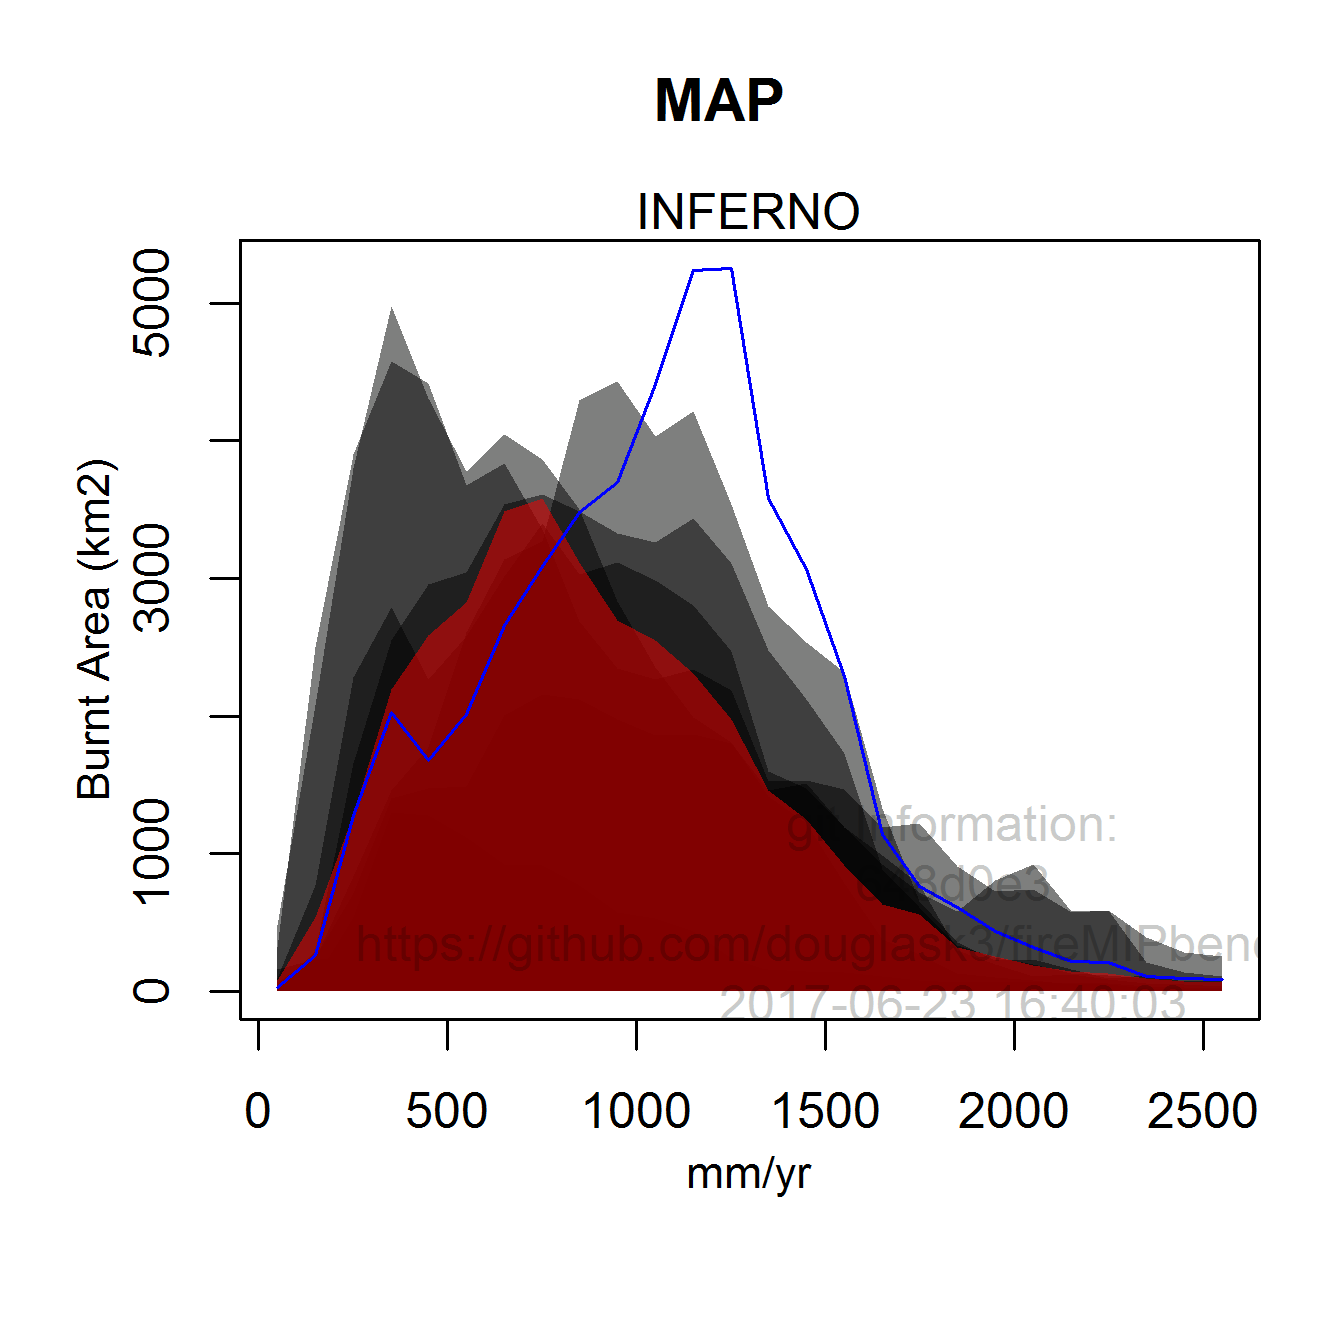
\includegraphics[width=4.8cm]{../../figs/burntArea_INFERNO_vs_MAP.png}	
		\end{textblock*}
	}
	\only<2->{
		\begin{textblock*}{14cm}(6.5cm,1.2cm)
			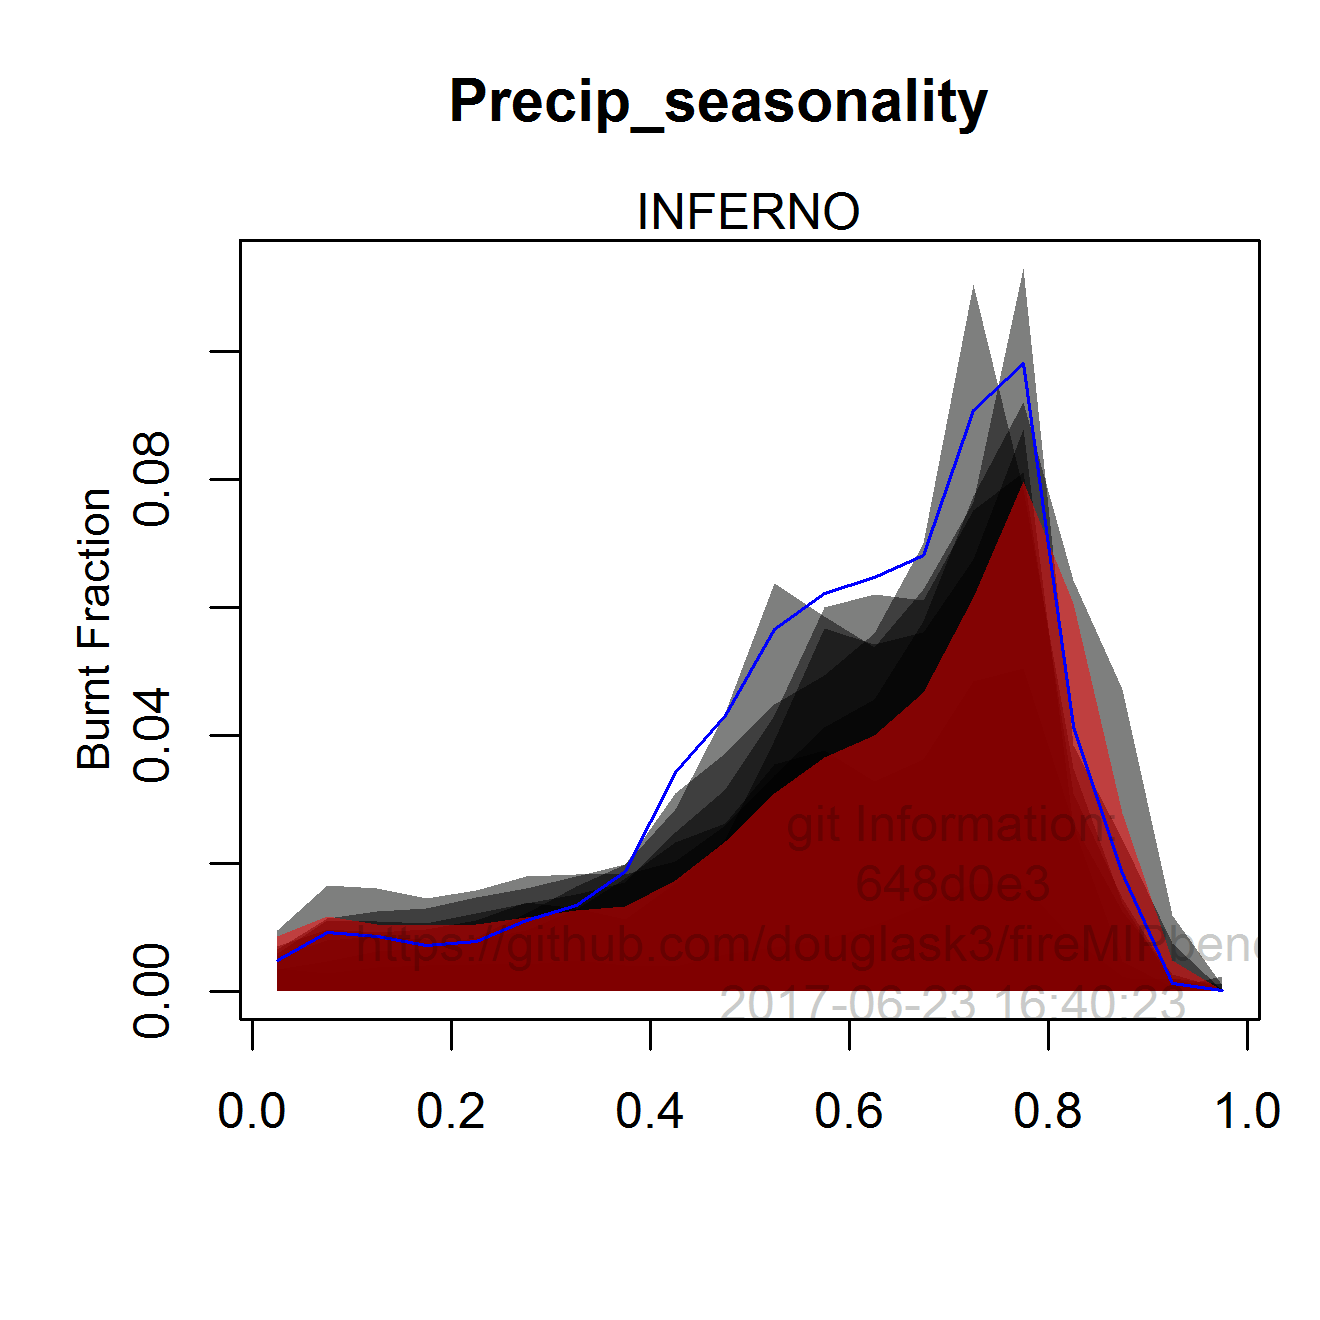
\includegraphics[width=4.8cm]{../../figs/burntArea_INFERNO_vs_Precip_seasonality.png}	
		\end{textblock*}
	}
	\only<3->{
		\begin{textblock*}{14cm}(3.4cm,4.5cm)
			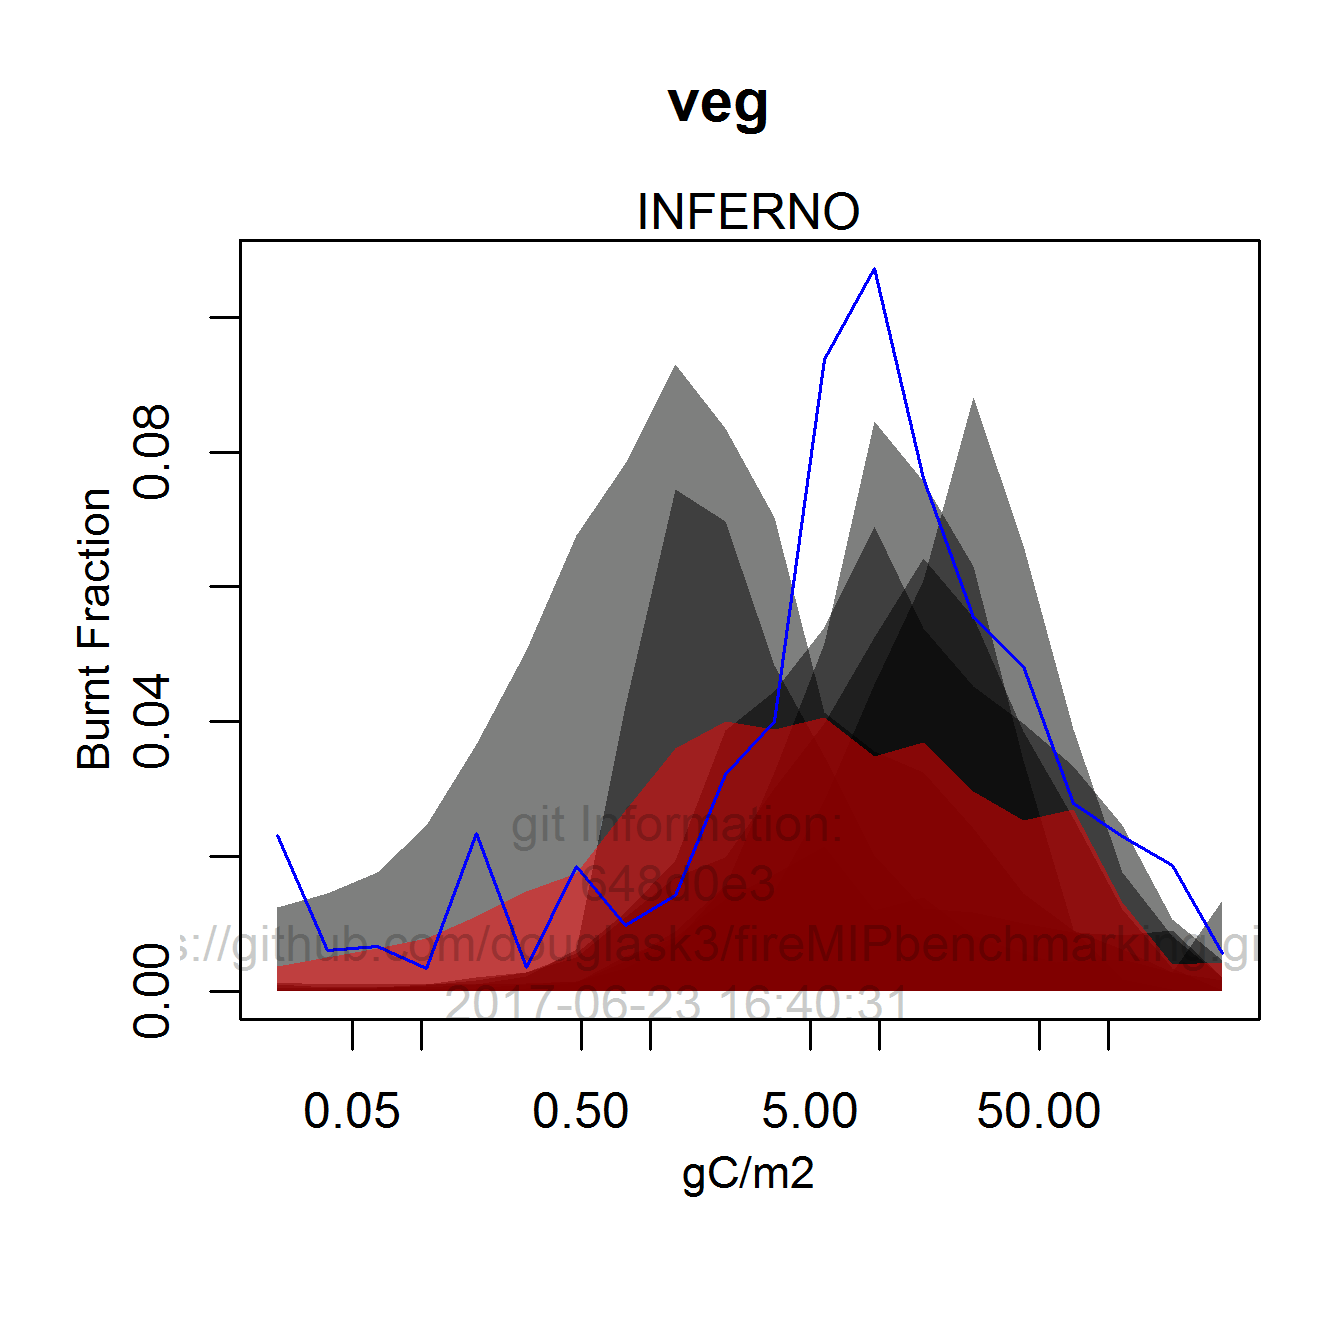
\includegraphics[width=4.8cm]{../../figs/burntArea_INFERNO_vs_veg.png}		
		\end{textblock*}
	}
	%\begin{textblock*}{14cm}(6.5cm,5.3cm)
	%	\includegraphics[width=5.78cm]{../diagrams/Logistic_fun.png}		
	%\end{textblock*}
\end{frame}

\pgfdeclareimage[width=1.0\paperwidth]{header-image}{header_images/Mirador_de_Garbi}

\begin{frame}[label = kelley2013Datasets]
	\frametitle{JULES-INFERNO v obs}
	\framesubtitle{Model scores}
	
	\begin{textblock*}{8cm}(11cm ,1.3cm)
		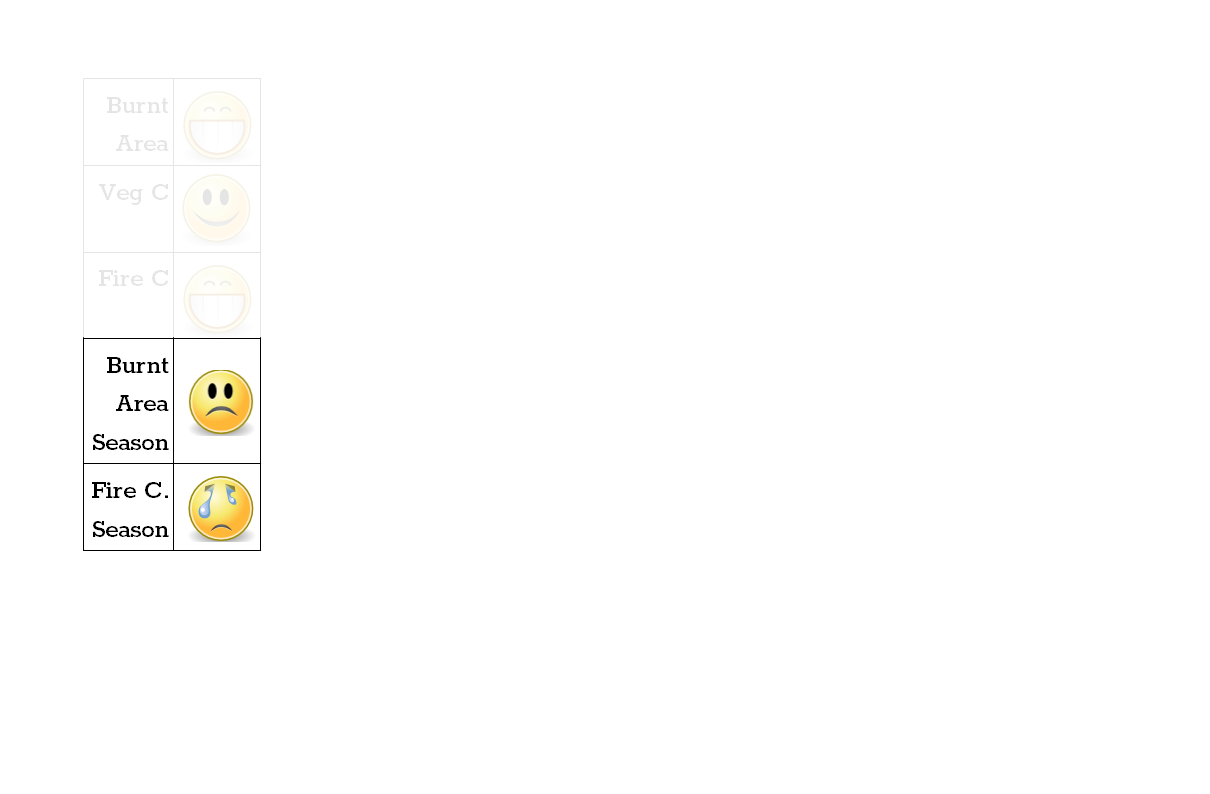
\includegraphics[width=7.5cm]{images/Smileys/BAFireCseason.png}
	\end{textblock*}
	
	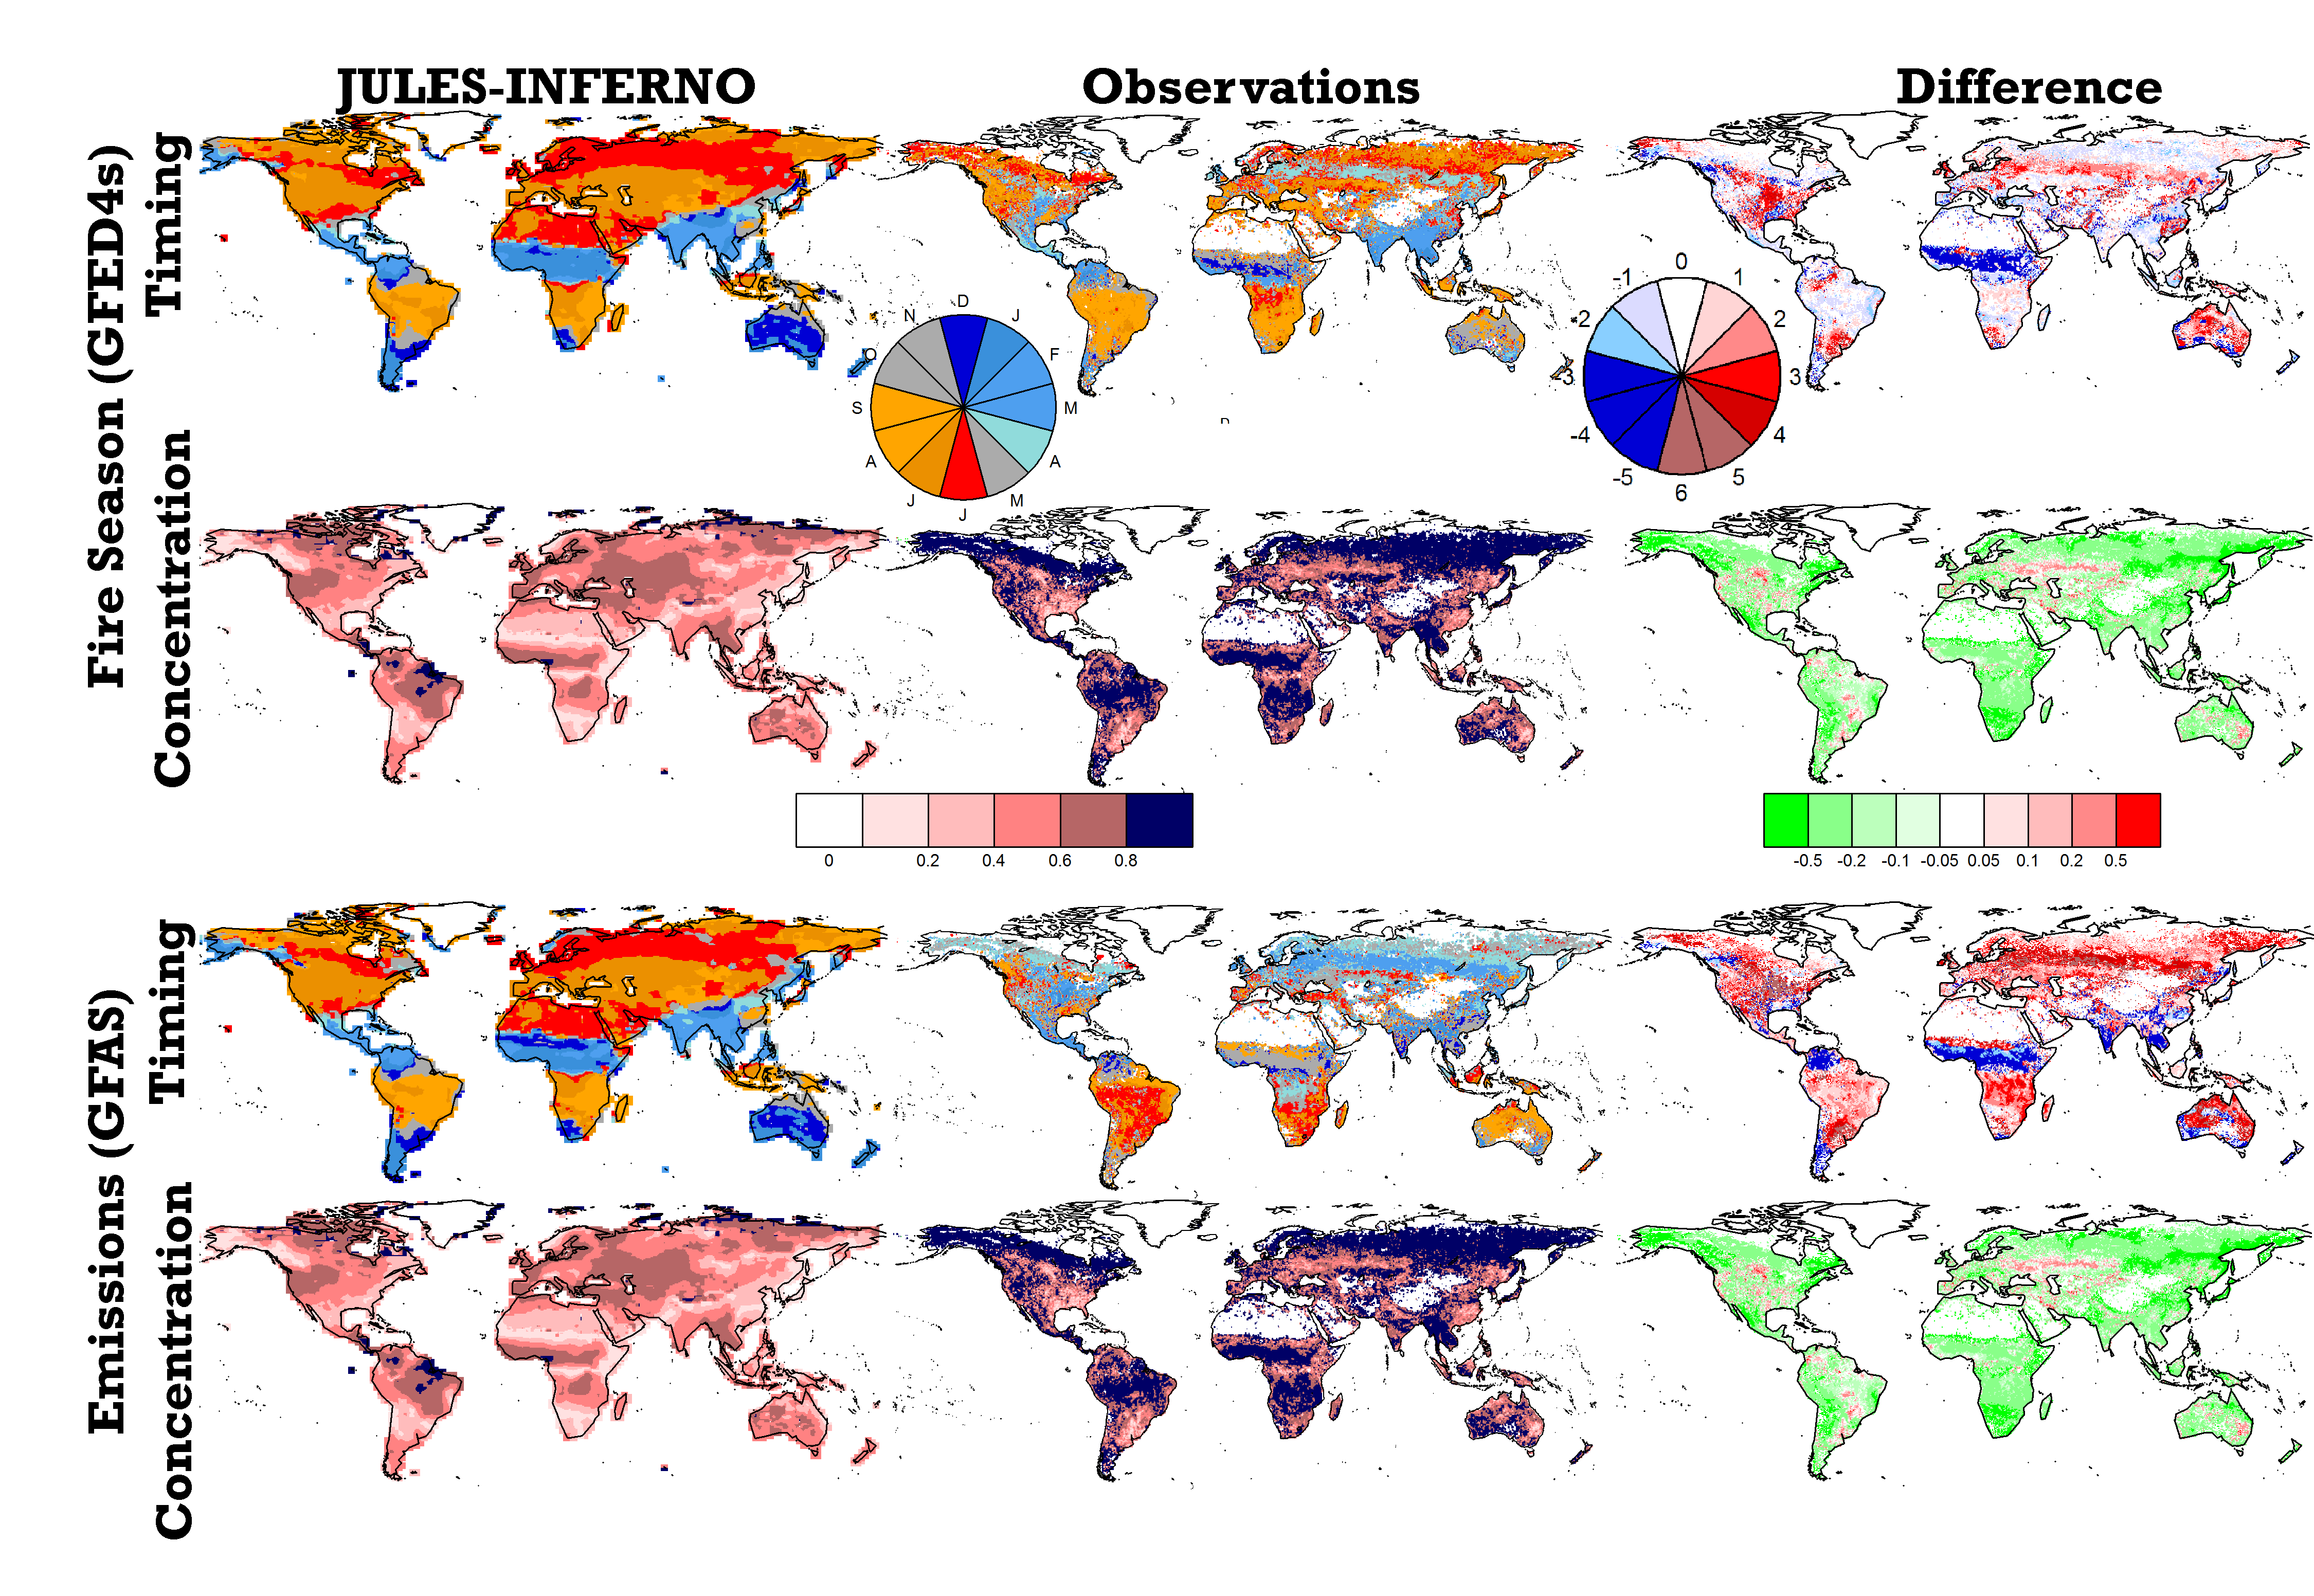
\includegraphics[width=10cm]{images/julesPerformance/FireMapsSeason.png}
	
\end{frame}

\begin{frame}[label = kelley2013Datasets]
	\frametitle{JULES-INFERNO v obs}
	\framesubtitle{Model scores}
	
	\begin{textblock*}{8cm}(11cm ,1.3cm)
		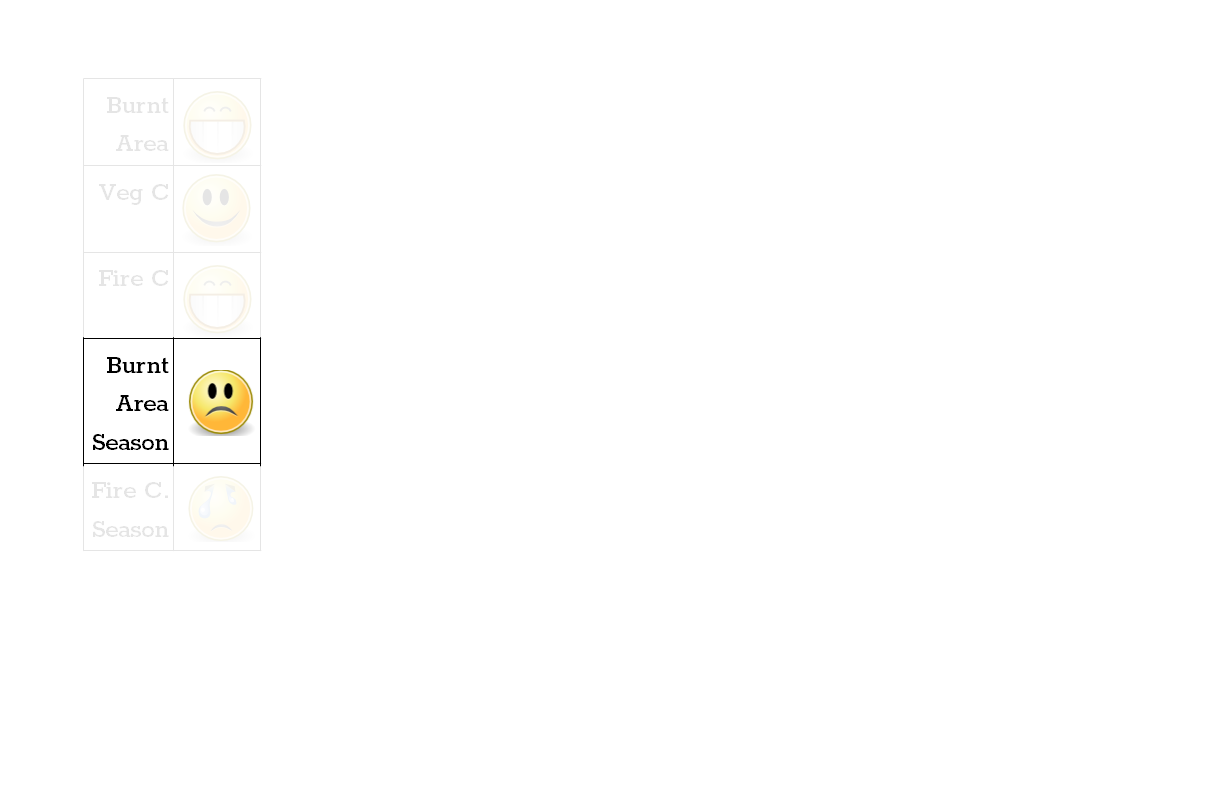
\includegraphics[width=7.5cm]{images/Smileys/BAseason.png}
	\end{textblock*}
	
	\begin{textblock*}{14cm}(0.5cm,2cm)
		\adjincludegraphics[trim={0 {.5\height} 0 0},clip, width=10cm]{../../figs/seasonality_JULES_normalised.png}
	\end{textblock*}
\end{frame}

%\begin{frame}[label = kelley2013Datasets]
%	\frametitle{Model type scores}
%	\framesubtitle{Model scores}
%	
%	% Model types scores
%\end{frame}

